
\documentclass{beamer}
\usepackage[utf8]{inputenc}
\usepackage[portuguese]{babel}

\usetheme{Szeged}


\title{Projeto Compiladores - Linguagem Lua}

\author{Fernando Da Rós e Leonardo Fiório Soares}

\institute[Universidade Federal Fluminense] 

\date{2017}

\begin{document}

\begin{frame}
  \titlepage
\end{frame}

\begin{frame}
        \frametitle{História da Linguagem Lua}
        Lua foi criada por um grupo de desenvolvedores da PUC-Rio com objetivo inicial de ser usada pela Petrobras. Devido à sua eficiência, clareza e facilidade de aprendizado, passou a ser usada em diversos ramos da programação. Hoje, a linguagem Lua é desenvolvida no laboratório LabLua do Departamento de Informática da própria PUC-Rio.

        \centering
        
\includegraphics[width=3cm]{images/lua.png}
\end{frame}

\begin{frame}
    \frametitle{Características da Linguagem Lua}
    
    \begin{itemize}
    \item Multiparadigma
    
         \begin{itemize}
            \item Procedural
            \item Orientada a Objetos
            \item Orientada a Dados
            \item Orientada a Descrição de Dados            
            \item \textbf{Funcional }
         \end{itemize}
    \end{itemize}
    \begin{itemize}
             \item Projetada para estender aplicações
                \begin{itemize}
                    \item Semântica extensível
                    \item Sua API se comunica com outras linguagens como C, C++, Java, C#, Smalltalk, Fortran...
                \end{itemize}        
     \end{itemize}
\end{frame}

\begin{frame}
    \frametitle{Características da Linguagem Lua}
    \begin{itemize}
        \item Lua oferece meta-mecanismos para construções na linguagem que sejam mais específicas. Isso ocorre sem que suas características básicas se percam.
        \item Simplicidade
        \item Portabilidade
            \begin{itemize}
                \item Para todas plataformas com compilador C
            \end{itemize}    
        \item Linguagem livre e de código aberto
    \end{itemize}
\end{frame}

\begin{frame}
    \frametitle{Características da Linguagem Lua}
    \begin{itemize}
        \item Tipagem Dinâmica: tipo da variável é definido quando o conteúdo é atribuído
         \item Favorece redigibilidade
         \item Pode dificultar procura por erros simples cometidos pelo programador
    \end{itemize}
\end{frame}

\begin{frame}
    \frametitle{Utilização da Linguagem Lua}
    \begin{itemize}
        \item Amplamente utilizada, principalmente na indústria de jogos, mas está presente também em outros softwares importantes e muito usados.
        \begin{columns}
            \begin{column}{5cm}
                
\includegraphics[width=5cm]{images/wow.jpg}
            \end{column}
            \begin{column}{4cm}
                
\includegraphics[width=3.5cm]{images/vlc.jpg}
            \end{column}
            \begin{column}{4cm}
                
\includegraphics[width=2.5cm]{images/mysql_workbench.png}
            \end{column}
        \end{columns}
    \end{itemize}
\end{frame}

\begin{frame}
    \frametitle{Processo de Compilação da Linguagem Lua}
        Linguagem interpretada\\
        
        Lua tem seu código fonte compilado gerando um bytecode que será interpretado pela máquina virtual baseada em registradores, garantindo sua portabilidade.
    
\end{frame}

\begin{frame}
    \frametitle{Estrutura da Linguagem Lua}
        Tipos 
            \begin{itemize}
                \item nil
                \item boolean
                \item string
                \item number (sempre ponto flutuante)
                \item function
                \item table
                \item thread
                \item userdata
            \end{itemize} 
\end{frame}


\begin{frame}
    \frametitle{Estrutura da Linguagem Lua}
     \begin{itemize}
        Palavras reservadas 
        \begin{columns}
            \begin{itemize}
            \begin{column}{5cm}
                \item and
                \item end
                \item in
                \item repeat
                \item break
                \item false
                \item local
                \item return
                \item do
                \item for
                \item nil
            \end{column}
            \begin{column}{5cm}
                \item then
                \item else
                \item function
                \item not
                \item true
                \item elseif
                \item if
                \item or
                \item until
                \item while
            \end{column}
            \end{itemize} 
        \end{columns}
    \end{itemize}
\end{frame}


\begin{frame}
    \frametitle{Exemplo de código}
    if a==1 then\\
        \begin{tabular} /print("variavel a é igual a 1")
        \end{tabular}\\
    end\\
    \newline
    cont = 1\\
    while cont <= 10 do\\
        \begin{tabular} /print(cont)\\
        cont = cont + 1
        \end{tabular}\\
    end
\end{frame}

\begin{frame}
    \frametitle{Vantagens da escolha}
    \begin{itemize} 
        \item Vantagens
        \begin{itemize}
            \item Simplicidade 
            \item Linguagem leve
            \item Existência de bibliotecas especializadas em pattern-matching
                \begin{itemize}
                    \item LPEG
                \end{itemize}
        \end{itemize}
        \item Desvantagens
        \begin{itemize}
            \item Possível falta de ferramentas específicas para de desenvolvimento de compiladores que auxiliem a programação
            \item Comparada a outras linguagens, pode aumentar o tempo necessário na busca de soluções para eventuais problemas devido ao menor número de comunidades
        \end{itemize}
    \end{itemize}
\end{frame}

\begin{frame}
    \frametitle{Vantagens da escolha - Exemplo Utilização LPEG}
    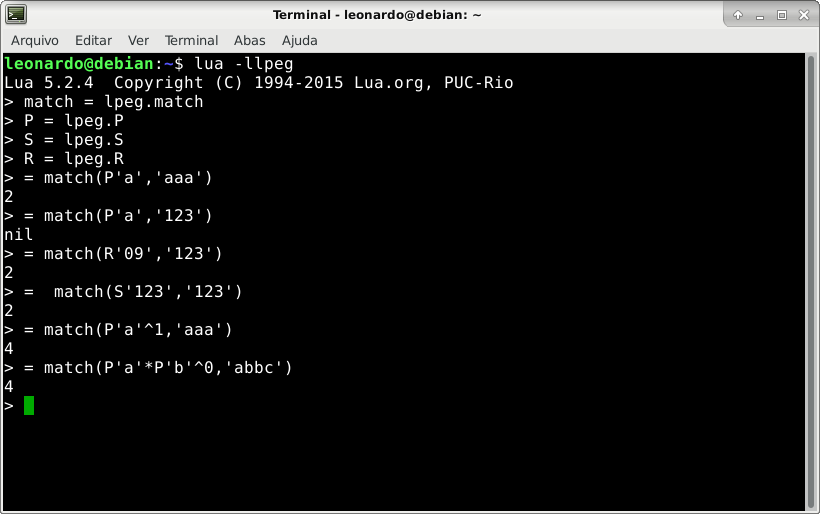
\includegraphics[width=10cm]{images/lpeg.png}
\end{frame}

\begin{frame}
    \frametitle{Principais comandos da biblioteca LPEG}
    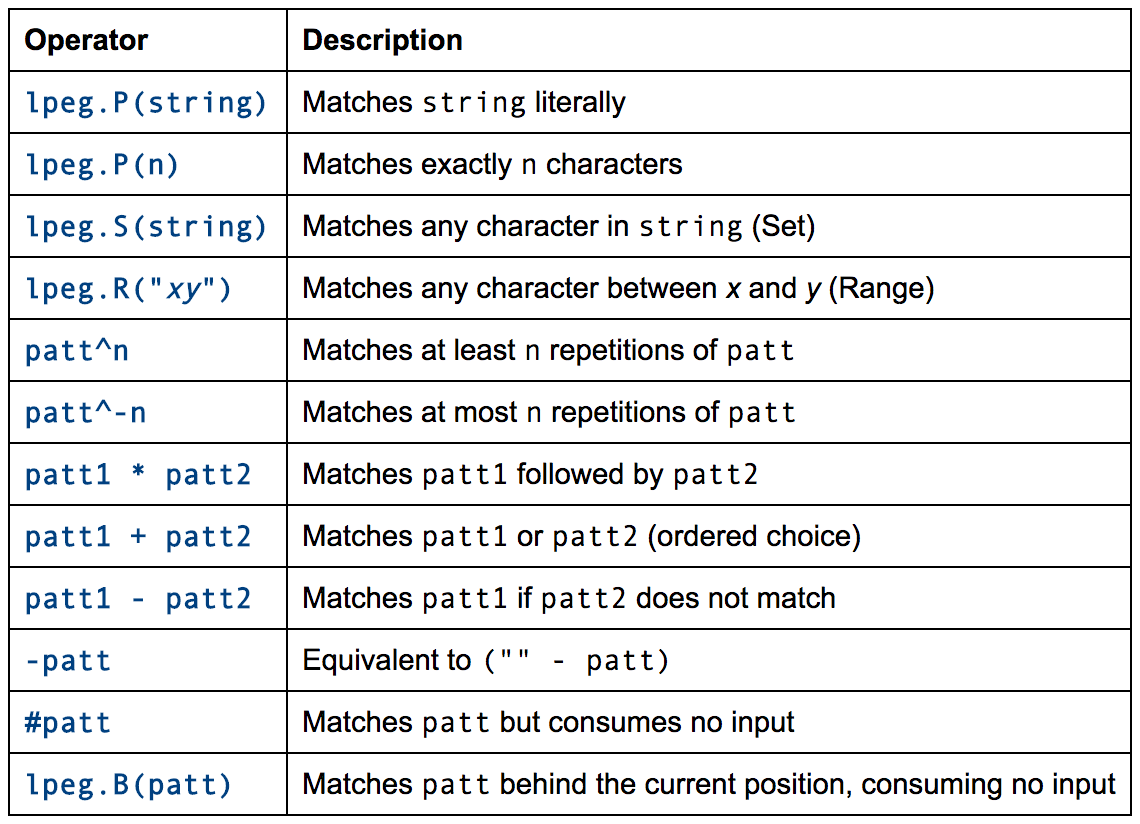
\includegraphics[width=10cm]{images/lpeg-commands.png}
\end{frame}

\begin{frame}
    \frametitle{Vantagens da escolha - Exemplo Utilização LPEG}
    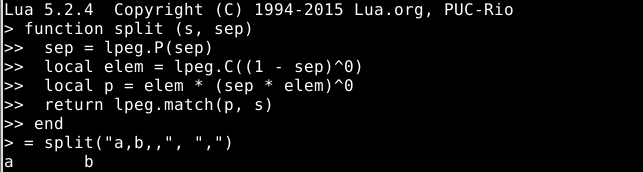
\includegraphics[width=10cm]{images/lpeg2.png}
    \begin{itemize}
        \item A biblioteca LPEG é uma ferramenta poderosa que permite sua utilização em gramáticas diferentes. 
        \item O exemplo acima ilustra a implementação de uma função que tem o objetivo de separar "pedaços" da expressão, a partir de um separador passado como parâmetro e uma expressão. 
    \end{itemize}
\end{frame}

\begin{frame}
    \titlepage{ Segunda Apresentação - Etapa de implementação de expressões e comandos }
\end{frame}

\begin{frame}
    \frametitle{Implementação de expressões e comandos}
    \begin{itemize}
        \item As estruturas de dados definidas foram:
        \begin{itemize}
            \item Pilha S
            \item Tabela M
            \item Pilha C
            \item Árvore (AST) 
            \begin{itemize}
                \item Possui tamanho variável, ou seja, é constituída por nós que tem uma lista de filhos
                \item Seus nós são do tipo node("data", \{ children \})
            \end{itemize}
        \end{itemize}
        \item As funções resolverExpressoes e resolverComandos são as responsáveis pela recursão sobre a árvore e executando o SMC
    \end{itemize}
\end{frame}


\begin{frame}
    \frametitle{Fatorial}
    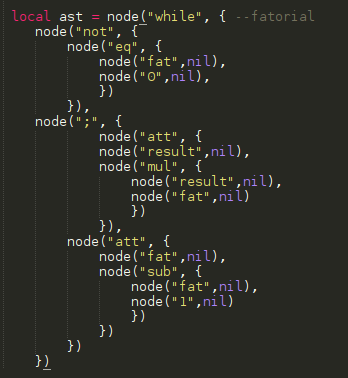
\includegraphics[width=5cm]{images/ast_fatorial.png}
    \centering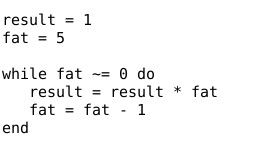
\includegraphics[width=5cm]{images/fatorial_normal.jpg}
\end{frame}

\begin{frame}
    Vamos ao código...
\end{frame}


\begin{frame}
    \frametitle{Referências}
    \begin{itemize}
        \item CELES, Waldemar. FIGUEIREDO, Luiz Henrique de. IERUSALIMSCHY, Roberto. A Linguagem Lua e suas Aplicações em Jogos. Disponível em https://www.lua.org/doc/wjogos04.pdf\  Acesso em 26 de Agosto de 2017.
        \item Página Oficial Linguagem Lua, A Linguagem de Programação Lua Disponível em https://www.lua.org/portugues.html. Acesso em 26 de Agosto de 2017.
        \item LEAL Marcus, Lua. Disponível em http://www.inf.puc-rio.br/~inf1621/lua1.pdf. Acesso em 26 de Agosto de 2017
    \end{itemize}
\end{frame}

\end{document}



